%%%%%%%%%%%%%%%%%%%%%%%%%%%%%%%%%%%%%%%%%%%%%%%%%%%%%%%%%%%%%%%%%%%%%%%%%%%%%%%%%%%%%%%%%%%%%%%%%%%
\subsection{Computing $P(Z < k)$ for Continuous Random Variables}

Even in the case where $X$ is purely a continuously distributed random variable functions such as $[X-k]^+$ may result in a mixed discrete and continuous random variable. In this section it is assumed that $X$ is continuous and $Z = f(X)$ is also continuous. The discrete and mixed cases will be addressed later.

%%%%%%%%%%%%%%%%%%%%%%%%%%%%%%%%%%%%%%%%%%%%%%%%%%%%%%%%%%%%%%%%%%%%%%%%%%%%%%%%%%%%%%%%%%%%%%%%%%%

\todo{XXX Rewrite the junk below}
%%%%%%%%%%%%%%%%%%%%%%%%%%%%%%%%%%%%%%%%%%%%%%%%%%%%%%%%%%%%%%%%%%%%%%%%%%%%%%%%%%%%%%%%%%%
\subsubsection{The Partition of the Domain of $f$}

The partition of $\mathcal{D}(X)$ induced by $Z^p$ through $f^{-1}$ is denoted $X^p$. Since $Z^p$ is composed of a finite number of elements, $X^p$ is similarly composed of a finite number of partition elements though the number of elements $m$ in $X^p$ may be larger than in $Z^p$. Except for a set of probability zero the partition elements of $X$ is a set of open intervals. 
\begin{figure}
  \centering
  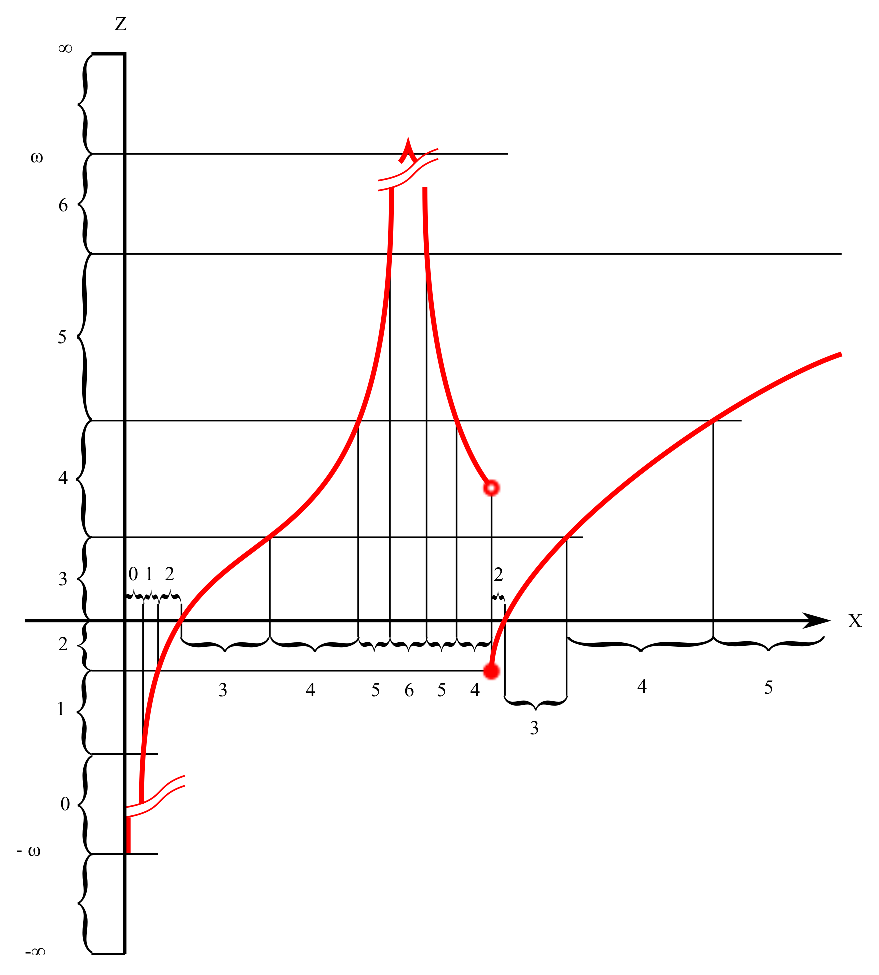
\includegraphics{Images/Exemplar_f.eps}
  \caption[Exemplar $f(x)$ with Indexed Partitions]
          {Exemplar $f(x)$ with Indexed Partitions}
  \label{fig:Exemplar_f}
\end{figure}

Refer to figure \ref{fig:Exemplar_f} for an example $f$ with labeled partition elements from an example $Z^{p+}$. Notice that the induced $X^p$ partition elements are given the associated $Z^{p+}$ partition element labels. Notice that some of the $Z^{p+}$ labels are duplicated. In particular the example $f$ seems to have a singularity in partition $6$. The algorithmic treatment of apparent singularities is detailed below. Finally, the example function $f$ is log-like and it appears $x \le 0$ is not in the domain of $f$. As with partition $6$, partition $0$ requires special consideration detailed below.

%%%%%%%%%%%%%%%%%%%%%%%%%%%%%%%%%%%%%%%%%%%%%%%%%%%%%%%%%%%%%%%%%%%%%%%%%%%%%%%%%%%%%%%%%%%
\subsection{Identifying $X^p$, the Extended Induced Partition of $\mathcal{D}(f^{-1}(Z))$}

Every Basic Random Variable in RICO has a \emph{suggested range} which can be used to choose a starting value $x_1 \in X$. 

\begin{figure}
  \centering
  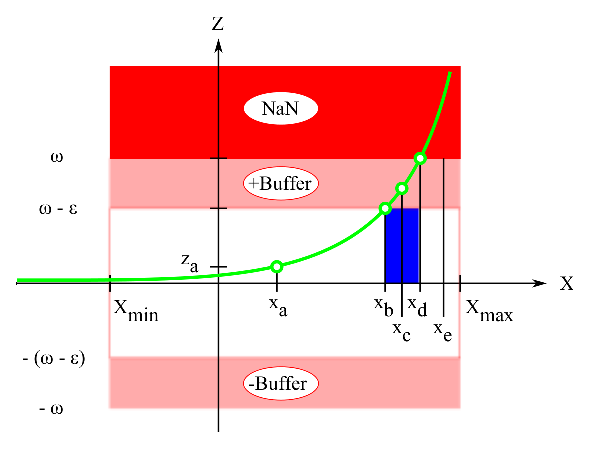
\includegraphics{Images/BoundExponential.eps}
  \caption[Exponential Function with Bounding Box]
          {Exponential Function with Bounding Box}
  \label{fig:BoundExponential}
\end{figure}

\todo{clean this up}
Figure \ref{fig:BoundExponential} exhibits some of the features that must be addressed by a numerical partition induction algorithm. Let $\omega$ be the largest number representable numerically i.e. as a floating point value. The RICO environment defines a value $\omega$ that is the largest value used as a partition endpoint. The reason for the $\omega$ choice is so that numerical any root finding algorithm will have the possibility of choosing values in the \emph{buffer zone} beteen $\omega$ and $\omega$ so that tangent lines and numeric \emph{overshoots} can be tolerated. The buffer zone is not intended to be large and as long as $P(x_b < X < x_d) \approx 0$ where $f(x_b) = \omega$ and $f(x_d) = \omega$ as in figure \ref{fig:BoundExponential} then the existence of the buffer zone is insignificant to the outcome.

Suppose that $Z^p = (-\omega, 0, \omega)$. Referring to figure \ref{fig:BoundExponential}, $P(-\omega < Z < 0) = 0$. To find the $P(0 < Z < \omega$ notice that the pre-image of the $(0, \omega)$ interval is the interval $(X_{min}, x_b)$. Initially (before any function evaluation) the pre-image is possibily the interval $(X_{min}, X_{max})$. To proceed the concept of \emph{bounding box} is introduced. A bounding box is the rectanglular subset of $(X,Z)$-space that represents the valid $X$- and $Z$-search limits. Initially the bounding box of the example in figure \ref{fig:BoundExponential} is $(-X_{min}, X_{max})\times(0, \omega)$ where the $Z$-limits are those of the given $Z^p$ partition element.

To find the pre-image limits of a $Z^p$ partition element a value in the pre-image is first located. Suppose the initial search value in \ref{fig:BoundExponential} is $x_a$. A left-search will reach the $X_{min}$ border of the associated bounding box and a right-search will reach the $\omega$ border at point $(x_b, \omega)$ and the pre-image is found to be $(X_{min}, x_b)$ so that
\begin{align*}
P(0 < Z < \omega) = P(X_{min} < X < x_b)
\end{align*}

Referring to figure \ref{fig:BoundExponential}, notice that $P(x_b < X)$ may be significant and no partition $Z^p$ will contain this \emph{lost probability}.

Suppose that instead of the initial search value $x_a$ being chosen in figure \ref{fig:BoundExponential} a point $x_c$ is chosen. The root-finding algorithm will search for $x_b$ and $x_d$ and RICO will record that interval $(x_b, x_d)$ is in the buffer zone. In RICO terminology the $(x_b, x_d)$ interval is \emph{explained}. This interval is shaded in figure \ref{fig:BoundExponential}. 

An important point is that the $X^P$-algorithm (pre-image identification) seeks to identify the pre-image intervals of each partition element in a given $Z^p$ by explaining the $(X_{min}, X_{max})$ interval. The general approach is to pick a value in an unexplained sub-interval, such as $(X_{min}, x_b)$, identify the associated $Z^p$ partition element and search left and right for a containing interval such that all points in that interval as associated with the same $Z^p$ partition element.

Many root-finding algorithm such as Newton's Method (see a numerical text such as Burden and Faires \cite{burden01}), will fail if a point such as $x_e$ is chosen as the initial value in figure \ref{fig:BoundExponential} because $f(x_e)$ does not evaluate to a real value. In many programming languages the result is represented by $NaN$, or Not A Number. In figure \ref{fig:BoundExponential} the nearest upper bound is $X_{max}$. Another $x$-value must be chosen until a real value of $f(x)$ is found. Suppose this next value is $x_c$. The above proceedure of identifying the related interval $(x_b, x_d)$ proceeds and now $x_e \in (x_d, X_{max})$. A practical stopping condition is if $P(x_d < X < X_{max}) \approx 0$. If no \emph{stop}, then the recursive algorithm applied to each sub-interval $(x_d, x_e)$ and $(x_e, X_{max})$ is the following bisection method pseudo-code
\begin{lstlisting}
DEFINE FUNCTION g(func = f, interval = (a,b))
Let x = (a + b) / 2
IF f(x) == NaN THEN
  IF P(a < X < x) == 0
    THEN a = x 
    ELSE call g(f, (a,x))
  IF P(x < X < b) == 0 
    THEN b = x
    ELSE call g(f, (x,b))
  IF a == b THEN stop
ELSE
  Let (c,d) be the associated interval of x
  call g(f, (d,b))
LOOP
\end{lstlisting}

The explaination algorithm begins with the unexplained interval $(X_{min}, X_{max})$. When the $x_c$ point is tested and the $(x_b, x_d)$ interval explained it subdivides the containing interval into three pieces: $(X_{min}, X_{max}) = (X_{min}, x_b) \cup (x_b, x_d) \cup (x_d, X_{max})$ the middle interval is moved the the \emph{explained list} and the other two intervals replace the original interval on the \emph{unexplained list}. The unexplained list is an ordered list of disjoint intervals.

\subsection{Addressing Apparent Singularities  of $f(x)$.}

